%                      Code_Saturne version 1.3
%                      ------------------------
%
%     This file is part of the Code_Saturne Kernel, element of the
%     Code_Saturne CFD tool.
%
%     Copyright (C) 1998-2007 EDF S.A., France
%
%     contact: saturne-support@edf.fr
%
%     The Code_Saturne Kernel is free software; you can redistribute it
%     and/or modify it under the terms of the GNU General Public License
%     as published by the Free Software Foundation; either version 2 of
%     the License, or (at your option) any later version.
%
%     The Code_Saturne Kernel is distributed in the hope that it will be
%     useful, but WITHOUT ANY WARRANTY; without even the implied warranty
%     of MERCHANTABILITY or FITNESS FOR A PARTICULAR PURPOSE.  See the
%     GNU General Public License for more details.
%
%     You should have received a copy of the GNU General Public License
%     along with the Code_Saturne Kernel; if not, write to the
%     Free Software Foundation, Inc.,
%     51 Franklin St, Fifth Floor,
%     Boston, MA  02110-1301  USA
%
%-----------------------------------------------------------------------
%

%%%%%%%%%%%%%%%%%%%%%%%%%%%%%%%%%%
%%%%%%%%%%%%%%%%%%%%%%%%%%%%%%%%%%
\section{Discr\'etisation}
%%%%%%%%%%%%%%%%%%%%%%%%%%%%%%%%%%
%%%%%%%%%%%%%%%%%%%%%%%%%%%%%%%%%%

\begin{figure}[h]
\parbox{8cm}{%
\centerline{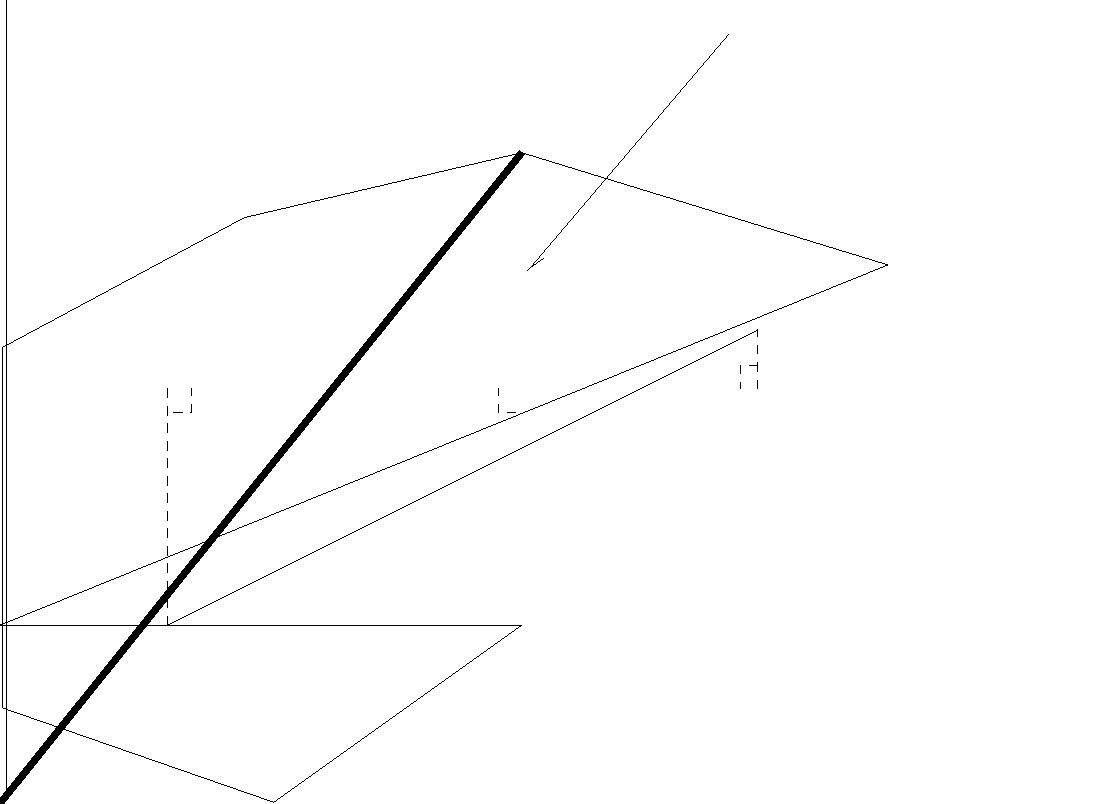
\includegraphics[height=4cm]{../Base/Matrix/Images/facette.pdf}}}
\parbox{8cm}{%
\centerline{
\includegraphics[height=4cm]{../Base/Matrix/Images/facebord.pdf}}}
\caption{\label{Base_Matrix_fig_geom_gradmc}D\'efinition des diff\'erentes entit\'es
g\'eom\'etriques pour les faces internes (gauche) et de bord (droite).}
\end{figure}

L'op\'erateur $\mathcal{EM_{\it{scal}}}$ s'\'ecrit, pour tout $I$ centre de cellule :
\begin{equation}
\begin{array}{lll}
\mathcal{EM_{\it{scal}}}(a,I) &=  f_s^{imp}\ a_I \\
&+\sum\limits_{j\in Vois(i)}\left[{(\rho \vect{u})_{\,ij}^n} \text{.}\, \vect{S}_{\,ij}\right]\ a_{\,f,ij}
+\sum\limits_{k\in {\gamma_b(i)}} \left[{(\rho \vect{u})_{\,{b}_{ik}}^n}
\text{.}\, \vect{S}_{\,{b}_{ik}}\right]\ {a_f}_{\,{b}_{ik}} \\
&-\sum\limits_{j\in Vois(i)} \beta_{\,ij}\displaystyle
\frac{a_{\,J}- a_{\,I}}{\overline{I'J'}} S_{\,ij}
-\sum\limits_{k\in {\gamma_b(i)}} \beta_{\,b_{ik}}\displaystyle
\frac{a_{\,b_{ik}}-a_{\,I}}{\overline{I'F}} S_{\,b_{ik}} \\
\end{array}
\end{equation}
o\`u
$a_{\,f,ij} = a_{\,I} \text{ ou }  a_{\,J}$
selon le signe de $(\rho \vect{u})_{\,ij}^n.\vect{S}_{\,ij}$ (sch�ma
convectif upwind syst�matique),
et avec $\overline{I'J'}$, mesure alg\'ebrique, orient\'ee comme la
normale sortante \`a la face, {\it i.e.} allant de $I$ vers $J$ pour la cellule
$\Omega_i$ de centre $I$. On la
notera ${\overline{I'J'}^{\tiny {\,I}}}$ lorsqu'on aura besoin d'expliciter
clairement l'orientation.\\
${a_f}_{\,{b}_{ik}} = a_I \text{ ou  }
a_{\ {b}_{ik}}$ selon le signe de
${(\rho \vect{u})_{\,{b}_{ik}}^n}\text{.}\, \vect{S}_{\,{b}_{ik}}$ (sch�ma
upwind syst�matique)
et $a_{\ {b}_{ik}}$ valeur au bord est donn\'ee directement par les conditions
aux limites (valeur non reconstruite). $\overline{I'F}$, mesure alg\'ebrique, orient\'ee relativement \`a la
normale sortante \`a la face, {\it i.e.} allant de $I$ vers l'ext\'erieur du domaine.\\
En g\'en\'eral, sauf cas pathologiques, les mesures alg\'ebriques
$\overline{I'J'}$ et $\overline{I'F}$
sont positives et correspondent aux distances $I'J'$ et $I'F$. On se reportera
au paragraphe Points \`a traiter pour plus de d\'etails.\\
Soit ${\tens{EM}}_{\,scal}$ la matrice associ\'ee ; sa taille est {\it a priori} de
$\var{NCEL} * \var{NCEL}$, mais compte-tenu de la nature de la structure de
donn\'ees, seuls deux tableaux \var{DA(NCEL)} contenant les valeurs
diagonales et \var{XA(NFAC,*)} les contributions des termes extra-diagonaux sont n\'ecessaires, avec \var{NCEL} nombre de
cellules du maillage consid\'er\'e et \var{NFAC} nombre de faces internes associ\'e.\\
Du fait des simplifications effectu\'ees sur la matrice (non reconstruction des
termes), les composantes extradiagonales de la ligne $I$ ne sont diff\'erentes de z\'ero que pour
les indices $J$ des cellules voisines de $I$. On peut donc stocker toutes les
contributions non nulles de la matrice dans deux tableaux \var{DA(NCEL)} et \var{XA(NFAC,2)} :\\
$\bullet$ \var{DA(I)} est le coefficient de la colonne $I$ dans la ligne $I$,\\
$\bullet$ si \var{IFAC} est une face qui s\'epare les cellules $\Omega_i$
et $\Omega_j$, orient\'ee de $I$ vers $J$, alors :\\
$\var{XA(IFAC,1)}$ est le coefficient de la colonne $J$ dans la ligne $I$ et
$\var{XA(IFAC,2)}$ est le coefficient de la colonne $I$ dans la ligne $J$.
Lorsque la matrice est sym\'etrique, {\it
i.e.} lorsqu'il n'y a pas de convection (\var{ICONVP} = 0) et que seule la
diffusion est \`a prendre en compte, alors $\var{XA(IFAC,1)} = \var{XA(IFAC,2)}
$ et on r\'eduit \var{XA} \`a $\var{XA(NFAC,1)}$.\\\\
Soit $m_{\,ij}^n$ (\ $m_{\,{b}_{ik}}^n$\ ) la valeur de $(\rho
\vect{u})_{\,ij}^n.\vect{S}_{\,ij}$ (respectivement $(\rho
\vect{u})_{\,{b}_{ik}}^n\text{.}\,\vect{S}_{\,{b}_{ik}}$).\\
Alors~:\\
\hspace*{1cm}{\tiny$\blacksquare$}\ \underline{contribution volumique} : $ f_s^{\,imp}\ a_I $\\\\
\hspace*{1cm}{\tiny$\blacksquare$}\ \underline{contribution d'une face purement interne $ij$} \\
L'expression \\
\begin{equation}\notag
+ \sum\limits_{j\in Vois(i)}{F^{\,amont}_{\,ij}((\rho \vect{u})^n, a)}
- \sum\limits_{j\in Vois(i)}{D^{NRec}_{\,ij}(\,\beta, a)}
\end{equation}
 s'\'ecrit :
\begin{equation}\label{Base_Matrix_eq_face_int}
\begin{array}{ll}
&\ \sum\limits_{j\in Vois(i)}\displaystyle\left({ \left[{(\rho \vect{u})_{\,ij}^n} \text{.}\,
\vect{S}_{\,ij}\right]\ \ a_{\,f,ij} - \beta_{\,ij}\frac{a_J - a_I}{\overline{I'J'}} S_{\,ij}}\right)\\
&=\sum\limits_{j\in Vois(i)}\left[\displaystyle\frac{1}{2}(\  m_{\,ij}^n + |\
m_{\,ij}^n|\ )\,a_I + \displaystyle\frac{1}{2}(\ m_{\,ij}^n - |\
m_{\,ij}^n|)\,a_J\right] - \sum\limits_{j\in Vois(i)}\displaystyle \beta_{\,ij}\frac{a_J - a_I}{\overline{I'J'}} S_{\,ij}
\end{array}
\end{equation}\\
Ici, $\overline{I'J'} = {\overline{I'J'}^{\tiny {\,I}}}$.\\\\
\hspace*{1cm}{\tiny$\blacksquare$}\ \underline{contribution d'une face de bord $ik$} \\
De m\^eme :
\begin{equation}\label{Base_Matrix_eq_face_bord}
\begin{array}{ll}
&\ \sum\limits_{k\in {\gamma_b(i)}} {F^{\,amont}_{\,{b}_{ik}}((\rho \vect{u})^n,a)}
- \sum\limits_{k\in {\gamma_b(i)}} {D^{NRec}_{\,{b}_{ik}}(\beta, a)}\\
&=\sum\limits_{k\in {\gamma_b(i)}}\displaystyle\left(\left[{(\rho
\vect{u})_{\,{b}_{ik}}^n} \text{.}\, \vect{S}_{\,{b}_{ik}}\right]\
{a_f}_{\,{b}_{ik}} - \beta_{\,b_{ik}}
\frac{a_{\,b_{ik}}- a_I}{\overline{I'F}} S_{\,b_{ik}}\right)\\
&=\sum\limits_{k\in {\gamma_b(i)}}\left[\displaystyle\frac{1}{2}(\ m_{\,{b}_{ik}}^n + |\ m_{\,{b}_{ik}}^n|\ )\,a_I +
\displaystyle\frac{1}{2}(\ m_{\,{b}_{ik}}^n -
|m_{\,{b}_{ik}}^n|)\,a_{\,{b}_{ik}}\right] - \sum\limits_{k\in {\gamma_b(i)}}\displaystyle\beta_{\,b_{ik}}
\frac{a_{\,b_{ik}}- a_I}{\overline{I'F}} S_{\,b_{ik}}
\end{array}
\end{equation}
avec~:
\begin{equation}\notag
a_{\,{b}_{ik}} = \var{INC}\,A_{\,b,ik} + B_{\,b,ik}\,a_I =  B_{\,b,ik}\,a_I
\end{equation}
$a$ n'\'etant associ\'ee qu'\`a des conditions aux limites de type Dirichlet
homog\`ene ou de type Neumann homog\`ene.

